%%%%%%%%%%%%%%%%%%%%%%%%%%%%%%%%%%%%%%%%%
% fphw Assignment
% LaTeX Template
% Version 1.0 (27/04/2019)
%
% This template originates from:
% https://www.LaTeXTemplates.com
%
% Authors:
% Class by Felipe Portales-Oliva (f.portales.oliva@gmail.com) with template 
% content and modifications by Vel (vel@LaTeXTemplates.com)
%
% Template (this file) License:
% CC BY-NC-SA 3.0 (http://creativecommons.org/licenses/by-nc-sa/3.0/)
%
%%%%%%%%%%%%%%%%%%%%%%%%%%%%%%%%%%%%%%%%%

%----------------------------------------------------------------------------------------
%	PACKAGES AND OTHER DOCUMENT CONFIGURATIONS
%----------------------------------------------------------------------------------------

\documentclass[
	12pt,
	%fleqn, % Default font size, values between 10pt-12pt are allowed
	%letterpaper, % Uncomment for US letter paper size
	%spanish, % Uncomment for Spanish
]{fphw}

% Template-specific packages
\usepackage[utf8]{inputenc} % Required for inputting international characters
\usepackage[T1]{fontenc} % Output font encoding for international characters
\usepackage{mathpazo} % Use the Palatino font

\usepackage{graphicx} % Required for including images

\usepackage{booktabs} % Required for better horizontal rules in tables

\usepackage{listings} % Required for insertion of code

\usepackage{enumerate} % To modify the enumerate environment

\usepackage{enumitem}

\usepackage{amsmath}

\usepackage{mathtools,amsthm}

\usepackage{float}

\usepackage{listings}

\usepackage{hyperref}

\usepackage{xcolor}

\usepackage{pdfpages}
\lstdefinelanguage{R}{
  keywords={if, else, repeat, while, function, for, in, next, break},
  otherkeywords={TRUE, FALSE, NULL, NA, Inf, NaN},
  sensitive=true,
  morecomment=[l]\#,
  morestring=[b]",
}

\newcommand{\E}{\mathbb{E}}
\newcommand{\Var}{\operatorname{Var}}
\newcommand{\R}{\mathbb{R}}
\newcommand{\norm}[1]{\left\lVert #1 \right\rVert}

%%better python code style
\definecolor{codebg}{RGB}{248,249,250}
\definecolor{codekw}{RGB}{30,64,175}
\definecolor{codestr}{RGB}{185,28,28}
\definecolor{codecom}{RGB}{22,101,52}
\definecolor{codenum}{RGB}{107,114,128}
\definecolor{codeframe}{RGB}{209,213,219}

\lstdefinestyle{pythonclean}{
    language=Python,
    basicstyle=\ttfamily\small,
    keywordstyle=\bfseries\color{codekw},
    stringstyle=\color{codestr},
    commentstyle=\itshape\color{codecom},
    identifierstyle=\color{black},
    showstringspaces=false,
    numbers=left,
    numberstyle=\scriptsize\color{codenum},
    numbersep=8pt,
    frame=single,
    framerule=0.6pt,
    rulecolor=\color{codeframe},
    backgroundcolor=\color{codebg},
    breaklines=true,
    breakatwhitespace=true,
    tabsize=4,
    keepspaces=true,
    xleftmargin=1em,
    xrightmargin=0.5em,
    aboveskip=1em,
    belowskip=1em
}
\lstset{style=pythonclean}


%----------------------------------------------------------------------------------------
%	ASSIGNMENT INFORMATION
%----------------------------------------------------------------------------------------

\title{Homework \#12} % Assignment title

\author{Shizhe Zhang} % Student name

\date{\today} % Due date

\institute{University of California, Berkeley \\ Department of Statistics} % Institute or school name

\class{EECS 227AT} % Course or class name

\professor{Gireeja Ranade} % Professor or teacher in charge of the assignment

%----------------------------------------------------------------------------------------

\begin{document}

\maketitle % Output the assignment title, created automatically using the information in the custom commands above

%----------------------------------------------------------------------------------------
%	ASSIGNMENT CONTENT
%----------------------------------------------------------------------------------------

\section*{Problem 1. Formulating problems as LPs or QPs}

Formulate the problem

\[
p^* = \min_{\vec{x}} f_j(\vec{x}),
\]

for different functions \(f_j\), \(j = 1, \ldots, 4\), as convex QPs or LPs, or, if you cannot, explain why. 
\\In our formulations, we always use \(\vec{x} \in \mathbb{R}^n\) as the variable, and assume that \(A \in \mathbb{R}^{m \times n}\), \(\vec{y} \in \mathbb{R}^m\). 
\\If you obtain a convex LP or QP formulation, state precisely what the variables, objective, and constraints are.

(a) \(f_1(\vec{x}) = \|A\vec{x} - \vec{y}\|_\infty + \|\vec{x}\|_1.\)

(b) \(f_2(\vec{x}) = \|A\vec{x} - \vec{y}\|_2^2.\)

(c) \(f_3(\vec{x}) = \|A\vec{x} - \vec{y}\|_2^2 + \|\vec{x}\|_2^2.\)

(d) \(f_4(\vec{x}) = \|A\vec{x} - \vec{y}\|_2^2 - \|\vec{x}\|_1.\)

\subsection*{Answer}

We analyze each function and determine whether it can be written as a linear program (LP) or a convex quadratic program (QP).

\textbf{(a)} \(f_1(x) = \|Ax - y\|_\infty + \|x\|_1.\)

Introduce auxiliary variables \(t\) and \(u_i\). The problem becomes

\[
\min_{x,t,u} \quad t + \sum_{i=1}^{n} u_i
\]

subject to

\[
-(Ax-y)_i \le t,\quad (Ax-y)_i \le t, \quad i=1,\dots,m
\]

\[
-x_i \le u_i,\quad x_i \le u_i, \quad i=1,\dots,n
\]

\[
u_i \ge 0.
\]

The objective is linear and all constraints are linear, so this is a LP.

\vspace{0.5em}

\textbf{(b)} \(f_2(x) = \|Ax-y\|_2^2.\)

Expanding,

\[
\|Ax-y\|_2^2 = (Ax-y)^\top(Ax-y)
= x^\top A^\top A x - 2y^\top A x + y^\top y.
\]

Thus

\[
\min_x \frac{1}{2}x^\top (2A^\top A)x + (-2A^\top y)^\top x + y^\top y.
\]

Since \(A^\top A \succeq 0\), the Hessian is positive semidefinite. Therefore this is a convex QP with no constraints.

\vspace{0.5em}

\textbf{(c)} \(f_3(x) = \|Ax-y\|_2^2 + \|x\|_2^2.\)

Expanding,

\[
\|Ax-y\|_2^2 + \|x\|_2^2
= x^\top(A^\top A + I)x -2y^\top A x + y^\top y.
\]

Thus the problem is

\[
\min_x \frac{1}{2}x^\top (2(A^\top A + I))x + (-2A^\top y)^\top x + y^\top y.
\]

Since \(A^\top A + I \succ 0\), the Hessian is positive definite. This is also a convex QP with no constraints.

\vspace{0.5em}

\textbf{(d)} \(f_4(x) = \|Ax-y\|_2^2 - \|x\|_1.\)

\(-\|x\|_1\) is concave. The sum of a convex function and a concave function is generally non-convex. Therefore the objective is not convex, and the problem cannot be formulated as a convex LP or QP.

%----------------------------------------------------------------------------------------
\newpage
\section*{Problem 2. A Slalom Problem}

A skier must slide from left to right by going through \(n\) parallel gates of known position \((x_i, y_i)\) and width \(c_i\), \(i = 1, \ldots, n\). The initial position \((x_0, y_0)\) is given, as well as the final one, \((x_{n+1}, y_{n+1})\). Before reaching the final position, the skier must go through gate \(i\) by passing between the points \((x_i, y_i - c_i/2)\) and \((x_i, y_i + c_i/2)\) for each \(i \in \{1, \ldots, n\}\).

Figure~\ref{fig:1} is an example and does not have the right value of \(n\) nor show the true \((x_i, y_i, c_i)\) values. Use values for \((x_i, y_i, c_i)\) from Table 1.

\begin{figure}[H]
\centering
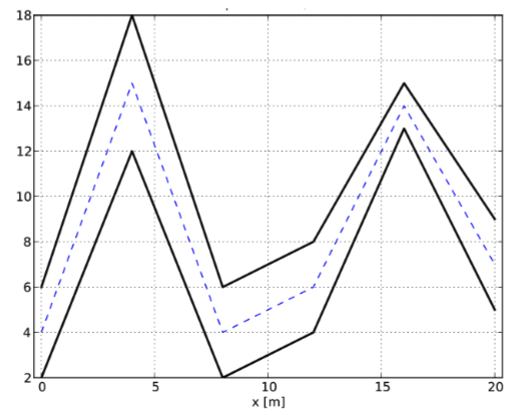
\includegraphics[width=0.6\textwidth]{figs/p2.png}
\caption{Slalom problem with \(n = 6\) gates. The initial and final positions are fixed and not included in the figure. The skier slides from left to right. The middle path is dashed and connects the center points of gates.}
\label{fig:1}
\end{figure}

Table 1: Problem data for Problem 2. Here \(n = 5\).

\[
\begin{array}{c|ccccccc}
i & 0 & 1 & 2 & 3 & 4 & 5 & 6 \\
\hline
x_i & 0 & 4 & 8 & 12 & 16 & 20 & 24 \\
y_i & 4 & 5 & 4 & 6 & 8 & 7 & 4 \\
c_i & \text{N/A} & 3 & 2 & 1 & 2 & 2 & \text{N/A}
\end{array}
\]

(a) Given the data \(\{(x_i, y_i, c_i)\}_{i=0}^{n+1}\), write an optimization problem that minimizes the total length of the path.

Your answer should come in the form of an SOCP.

(b) Solve the problem numerically with the data given in Table 1. HINT: You should be able to use packages such as cvxpy and numpy.

\subsection*{Answer}

\textbf{(a)}

The horizontal positions of the gates are fixed at \(x_i\).  
Each gate \(i\) has center height \(y_i\) and width \(c_i\).

Let the decision variable
$ z_i $ be the vertical coordinate where the skier crosses gate \(i\).

Thus the point where the skier passes gate \(i\) is

\[
p_i = (x_i, z_i).
\]

The skier must pass within the gate opening:

\[
y_i - \frac{c_i}{2} \le z_i \le y_i + \frac{c_i}{2},
\qquad i=1,\dots,n.
\]

The start and end points are fixed:

\[
p_0 = (x_0,y_0), \qquad p_{n+1}=(x_{n+1},y_{n+1}).
\]

The total path length is

\[
\sum_{i=0}^{n} \|p_{i+1}-p_i\|_2
=
\sum_{i=0}^{n}
\left\|
\begin{bmatrix}
x_{i+1}-x_i \\
z_{i+1}-z_i
\end{bmatrix}
\right\|_2.
\]

Introduce auxiliary variables \(t_i\) representing the length of each segment.

The optimization problem becomes

\[
\min_{z_1,\dots,z_n,\,t_0,\dots,t_n}
\sum_{i=0}^{n} t_i
\]

subject to the second–order cone constraints

\[
\left\|
\begin{bmatrix}
x_{i+1}-x_i \\
z_{i+1}-z_i
\end{bmatrix}
\right\|_2
\le t_i,
\qquad i=0,\dots,n
\]

and the gate constraints

\[
y_i - \frac{c_i}{2} \le z_i \le y_i + \frac{c_i}{2},
\qquad i=1,\dots,n.
\]

The start and end heights are fixed:

\[
z_0 = y_0, \qquad z_{n+1}=y_{n+1}.
\]

Each constraint

\[
\left\|
\begin{bmatrix}
x_{i+1}-x_i \\
z_{i+1}-z_i
\end{bmatrix}
\right\|_2
\le t_i
\]

is a second-order cone constraint, therefore the problem is an **SOCP**.

\bigskip

\textbf{(b) Numerical solution}

\begin{lstlisting}[language=Python]
import cvxpy as cp
import numpy as np
import matplotlib.pyplot as plt

# Problem data (Table 1)
x = np.array([0, 4, 8, 12, 16, 20, 24])
y = np.array([4, 5, 4, 6, 8, 7, 4])
c = np.array([None, 3, 2, 1, 2, 2, None], dtype=object)

n = 5  # number of gates

# Decision variables (crossing heights)
z = cp.Variable(n)

# Segment lengths
t = cp.Variable(n+1)

constraints = []

# Gate constraints
for i in range(1, n+1):
    constraints += [
        z[i-1] >= y[i] - c[i]/2,
        z[i-1] <= y[i] + c[i]/2
    ]

# Full vector including start/end
z_full = cp.hstack([y[0], z, y[-1]])

# SOCP constraints for path segments
for i in range(n+1):
    dx = x[i+1] - x[i]
    dy = z_full[i+1] - z_full[i]
    constraints.append(cp.norm(cp.hstack([dx, dy]), 2) <= t[i])

# Objective: minimize total path length
objective = cp.Minimize(cp.sum(t))

problem = cp.Problem(objective, constraints)
problem.solve()

# Build full path
z_opt = np.hstack([y[0], z.value, y[-1]])

# Plot
plt.figure(figsize=(8,4))

# Plot gates
for i in range(1, n+1):
    plt.plot([x[i], x[i]], [y[i]-c[i]/2, y[i]+c[i]/2], 'k', linewidth=4)

# Plot path
plt.plot(x, z_opt, '-o', label="Optimal path")

# Plot gate centers
plt.plot(x, y, '--', label="Gate centers")

plt.xlabel("x")
plt.ylabel("y")
plt.legend()
plt.title("Optimal Slalom Path")
plt.show()
\end{lstlisting}

\begin{figure}[H]
\centering
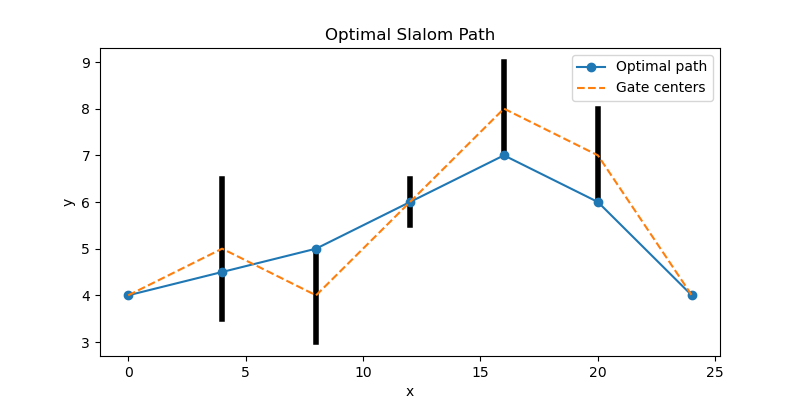
\includegraphics[width=0.8\textwidth]{figs/slalom_path.png}
\caption{Optimal slalom path}
\label{fig:slalom_path}
\end{figure}

Optimal path length: 24.90371052564722

Optimal crossing heights: [4.50009188 4.99999971 6.00001167 7.00000001 6.00000015]

%----------------------------------------------------------------------------------------
\newpage
\section*{Problem 3. Dual Norms and SOCP}

Consider the problem

\[
p^* = \min_{\vec{x} \in \mathbb{R}^n} \|A\vec{x} - \vec{y}\|_1 + \mu \|\vec{x}\|_2,
\]

where \(A \in \mathbb{R}^{m \times n}\), \(\vec{y} \in \mathbb{R}^m\), and \(\mu > 0\).

(a) Express this (primal) problem in standard SOCP form. HINT: you can make the objective function linear by introducing slack variables.

(b) Find a dual to the problem and express it in standard SOCP form. HINT: You may find Problem 1 in Discussion 13 to be helpful. Recall that for every vector \(\vec{z}\), the following dual norm equalities hold:

\[
\|\vec{z}\|_2 = \max_{\vec{u} : \|\vec{u}\|_2 \le 1} \vec{u}^\top \vec{z},
\]

\[
\|\vec{z}\|_1 = \max_{\vec{u} : \|\vec{u}\|_\infty \le 1} \vec{u}^\top \vec{z}.
\]

Additionally, you may use the following fact: If the primal problem is expressed as

\[
p^* = \min_{\vec{x}} \max_{\vec{y}} L(\vec{x}, \vec{y}),
\]

then the dual problem can be obtained by swapping the max and min:

\[
d^* = \max_{\vec{y}} \min_{\vec{x}} L(\vec{x}, \vec{y}).
\]

(c) Assume strong duality holds and that \(m = 100\) and \(n = 10^6\), i.e., \(A\) is \(100 \times 10^6\). Which problem would you choose to solve using a numerical solver: the primal or the dual? Justify your answer.

\subsection*{Answer}

\textbf{(a)}

Introduce auxiliary variables:
\[
t_i \ge |(Ax-y)_i|, \quad i=1,\dots,m,
\]
and
\[
s \ge \|x\|_2 .
\]

Then the objective becomes linear:

\[
\min_{x,t,s} \sum_{i=1}^m t_i + \mu s.
\]

The constraints are

\[
-(Ax-y)_i \le t_i, \quad (Ax-y)_i \le t_i, \quad i=1,\dots,m,
\]

\[
\|x\|_2 \le s.
\]

Thus the SOCP formulation is

\[
\min_{x,t,s} \sum_{i=1}^m t_i + \mu s
\]

subject to

\[
-(Ax-y)_i \le t_i, \quad (Ax-y)_i \le t_i, \quad i=1,\dots,m,
\]

\[
\|x\|_2 \le s.
\]

The last constraint is a second–order cone constraint, so the problem is an SOCP.

\bigskip

\textbf{(b) Dual problem}

Using dual norm identities,

\[
\|z\|_1 = \max_{\|u\|_\infty \le 1} u^\top z,
\]

\[
\|x\|_2 = \max_{\|v\|_2 \le 1} v^\top x.
\]

Apply this to the objective:

\[
\|Ax-y\|_1 + \mu \|x\|_2
=
\max_{\|u\|_\infty \le 1} u^\top(Ax-y)
+
\max_{\|v\|_2 \le 1} \mu v^\top x.
\]

Combine the maximizations:

\[
=
\max_{\|u\|_\infty \le 1,\ \|v\|_2 \le 1}
\left[
u^\top(Ax-y) + \mu v^\top x
\right].
\]

Thus

\[
p^* =
\min_x
\max_{\|u\|_\infty \le 1,\|v\|_2 \le 1}
\left[
x^\top(A^\top u + \mu v) - u^\top y
\right].
\]

Swap min and max to form the dual:

\[
d^* =
\max_{\|u\|_\infty \le 1,\|v\|_2 \le 1}
\min_x
\left[
x^\top(A^\top u + \mu v) - u^\top y
\right].
\]

The inner minimization over \(x\) is finite only if

\[
A^\top u + \mu v = 0.
\]

Thus

\[
v = -\frac{1}{\mu}A^\top u.
\]

Since \(\|v\|_2 \le 1\),

\[
\|A^\top u\|_2 \le \mu.
\]

Substituting back, the dual becomes

\[
\max_{u} -y^\top u
\]

subject to

\[
\|u\|_\infty \le 1,
\]

\[
\|A^\top u\|_2 \le \mu.
\]

This can be written as an SOCP:

\[
\max_u -y^\top u
\]

subject to

\[
-1 \le u_i \le 1, \quad i=1,\dots,m,
\]

\[
\|A^\top u\|_2 \le \mu.
\]

\bigskip

\textbf{(c) Which problem to solve}

Given

\[
m = 100, \quad n = 10^6,
\]

the primal problem has \(n=10^6\) variables \(x\), which is extremely large.

The dual problem instead has only \(m=100\) variables \(u\).

Therefore solving the dual problem is much more efficient numerically.

%----------------------------------------------------------------------------------------
\newpage
\section*{Problem 4. An illumination problem}

We consider an illumination system of \(m\) lamps, at positions \(\vec{l}_1, \ldots, \vec{l}_m \in \mathbb{R}^2\), illuminating \(n\) flat patches.

\begin{figure}[H]
\centering
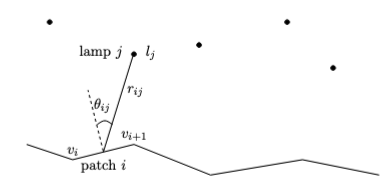
\includegraphics[width=0.65\textwidth]{figs/p4.png}
\end{figure}

The patches are line segments; the \(i\)th patch is given by \([\vec{v}_i, \vec{v}_{i+1}]\) where \(\vec{v}_1, \ldots, \vec{v}_{n+1} \in \mathbb{R}^2\). The variables in the problem are the lamp powers \(p_1, \ldots, p_m\), which can vary between 0 and 1.

The illumination at (the midpoint of) patch \(i\) is denoted \(I_i\). We will use a simple model for the illumination:

\[
I_i = \sum_{j=1}^{m} a_{ij} p_j,
\]

\[
a_{ij} = r_{ij}^{-2} \max\{\cos \theta_{ij}, 0\},
\]

where \(r_{ij}\) denotes the distance between lamp \(j\) and the midpoint of patch \(i\), and \(\theta_{ij}\) denotes the angle between the upward normal of patch \(i\) and the vector from the midpoint of patch \(i\) to lamp \(j\).

This model takes into account “self-shading” (i.e., the fact that a patch is illuminated only by lamps in the halfspace it faces) but not shading of one patch caused by another.

The problem is to determine lamp powers that make the illumination levels close to a given desired illumination level \(I_{des}\), subject to the power limits \(0 \le p_i \le 1\).

\begin{enumerate}
  \item[(a)]  Suppose we use the maximum deviation

\[
\phi(p) = \max_{k=1,\ldots,n} |I_k - I_{des}|
\]

as a measure for the deviation from the desired illumination level. Formulate the illumination problem using this criterion as a linear programming problem.
  
\item[(b)] There are several suboptimal approaches based on weighted least-squares. We consider two examples.

(i) Saturated least-squares. We can solve the least-squares problem

\[
\min \sum_{k=1}^{n} (I_k - I_{des})^2
\]

ignoring the constraints. If the solution is not feasible, we saturate it, i.e., set \(p_j := 0\) if \(p_j \le 0\) and \(p_j := 1\) if \(p_j \ge 1\).

Complete the \href{https://colab.research.google.com/drive/1nqA5k8SXVM8lcAzPEK3Txp4BbbHUiSit?usp=sharing}{notebook} and compute a feasible \(p\) using this method, and calculate \(\phi(p)\).

(ii) Weighted least-squares. We consider another least-squares problem:

\[
\min \sum_{k=1}^{n} (I_k - I_{des})^2 + \mu \sum_{i=1}^{m} (p_i - 0.5)^2.
\]
For large enough $\mu$, the solution of this problem will satisfy $0 \le p_i \le 1$ for all $i$, 
i.e., be feasible for the original problem. Complete the notebook and find the smallest $\mu$ such that $p$
becomes feasible, and evaluate $\phi(p)$.

\item[(c)] Complete the \href{https://colab.research.google.com/drive/1nqA5k8SXVM8lcAzPEK3Txp4BbbHUiSit?usp=sharing}{notebook}. Solve the LP you derived in part (a). Compare the solution with the solutions you
obtained using the (weighted) least-squares methods of part (b).

\end{enumerate}


\subsection*{Answer}

\paragraph{(a)}

The deviation measure is
\[
\phi(p) = \max_{k=1,\ldots,n} |I_k - I_{des}|.
\]

Introduce an auxiliary variable $t$ representing the maximum deviation.  
The problem becomes

\[
\begin{aligned}
\min_{p,t} \quad & t \\
\text{s.t.}\quad 
& -t \le I_k - I_{des} \le t, \qquad k=1,\ldots,n \\
& 0 \le p_j \le 1, \qquad j=1,\ldots,m .
\end{aligned}
\]

Since $I = Ap$, this can be written as

\[
\begin{aligned}
\min_{p,t} \quad & t \\
\text{s.t.}\quad 
& -t\mathbf{1} \le Ap - I_{des}\mathbf{1} \le t\mathbf{1}, \\
& 0 \le p \le 1 .
\end{aligned}
\]

This is a linear program since both the objective and constraints are linear.

%------------------------------------------------

\paragraph{(b)(i) Saturated least-squares}

Ignoring the box constraints, we first solve the least-squares problem

\[
\min_p \|Ap - I_{des}\mathbf{1}\|_2^2 .
\]

The optimal unconstrained solution is given by the normal equations

\[
p^{ls} = (A^TA)^{-1}A^T(I_{des}\mathbf{1}),
\]

assuming $A^TA$ is invertible.

%------------------------------------------------

\paragraph{(b)(ii) Weighted least-squares}

We now solve

\[
\min_p \|Ap - I_{des}\mathbf{1}\|_2^2 + \mu\|p - \dfrac{1}{2}\cdot \mathbf{1}\|_2^2 .
\]

\[
2A^T(Ap - I_{des}\mathbf{1}) + 2\mu(p - \dfrac{1}{2} \cdot \mathbf{1}) = 0.
\]

\[
p =
(A^TA + \mu I)^{-1}
\left(A^T(I_{des}\mathbf{1}) + \frac{\mu}{2} \cdot  \mathbf{1}\right).
\]

If desired, the final solution can again be projected to the feasible set
$0 \le p \le 1$.

The resulting illumination is

\[
I = Ap
\]

and the deviation is

\[
\phi(p) = \max_{k=1,\ldots,n} |I_k - I_{des}|.
\]

% insert the pdf notebook link here

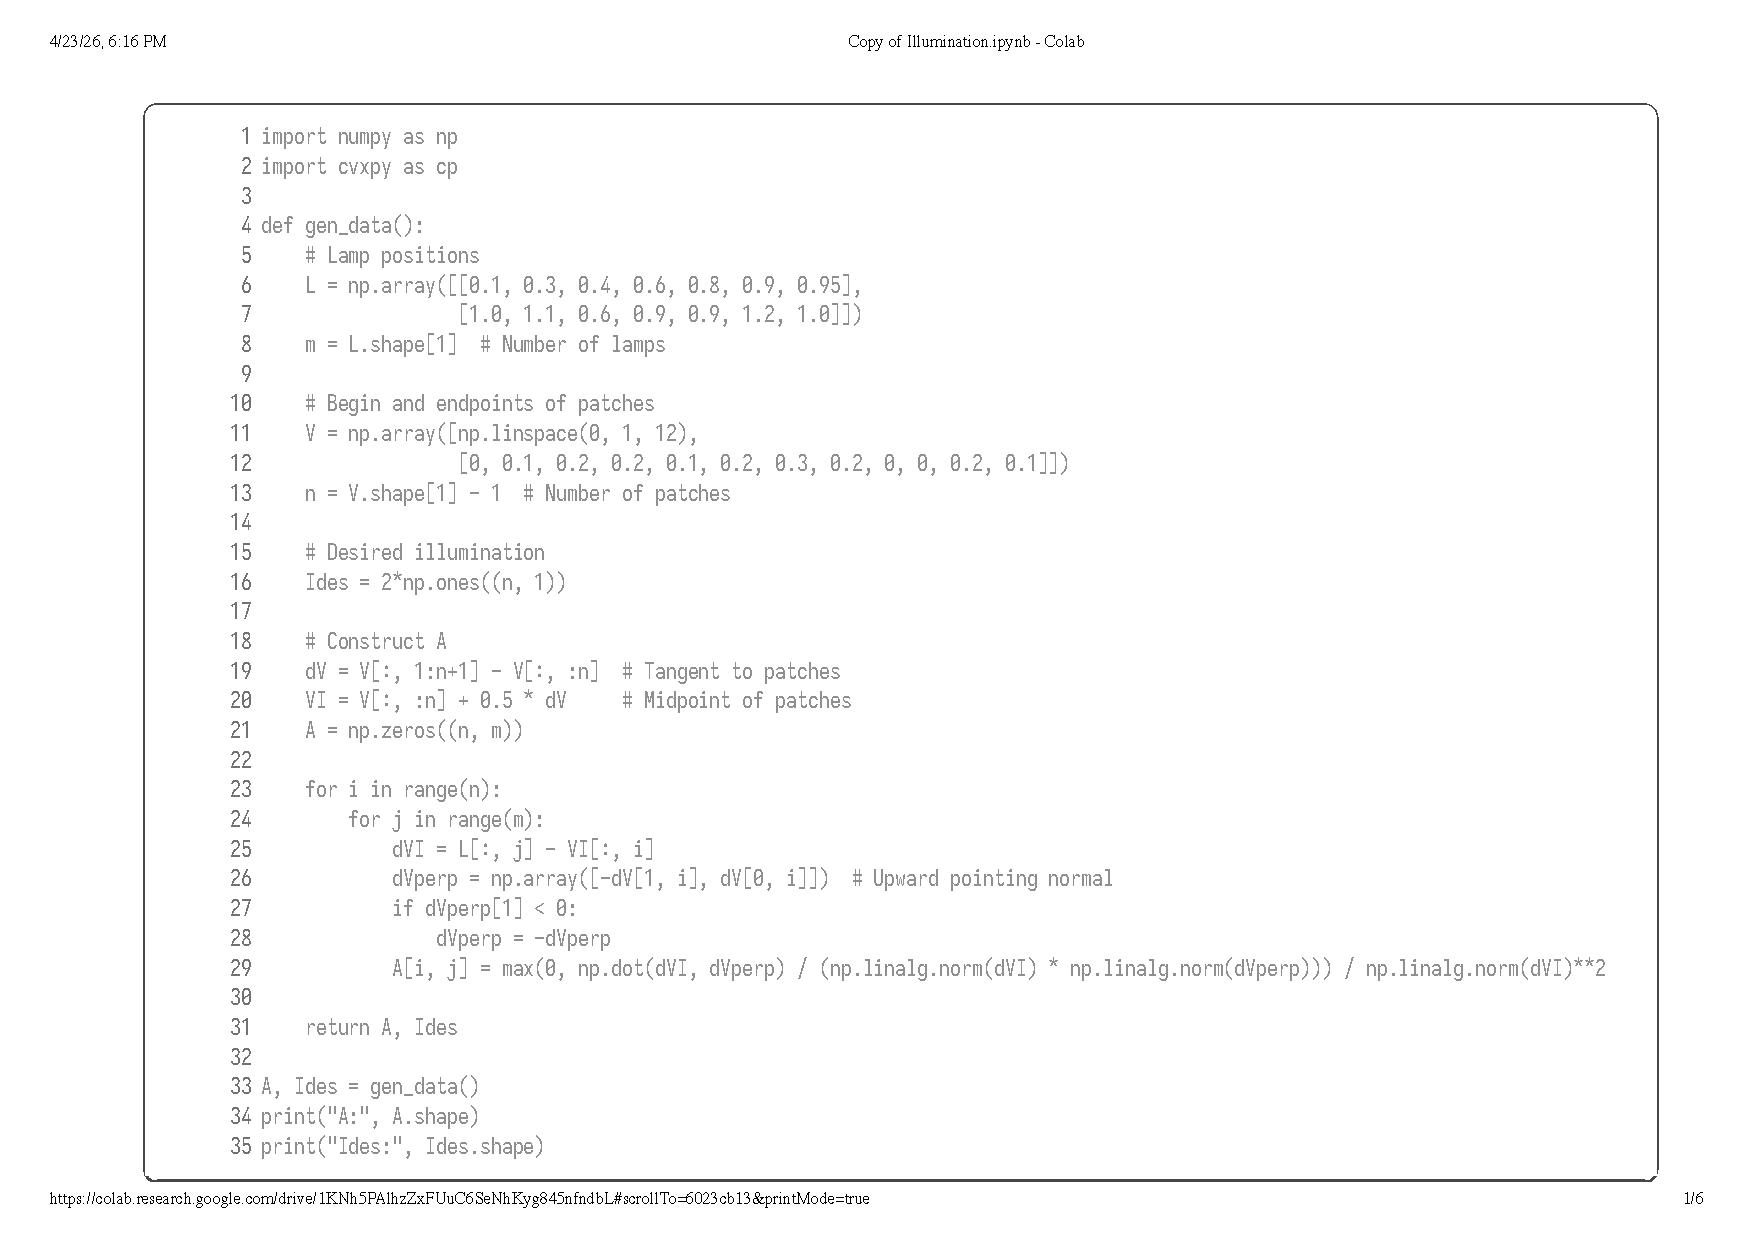
\includepdf[pages=-]{Illumination.pdf}


%----------------------------------------------------------------------------------------

\section*{Problem 5. Learning a Piecewise Constant Function}

A piecewise constant function is one that remains constant on intervals and may change values at specific points called \textbf{kinks}. 
Formally, it can be written as:

\[
f(x) =
\begin{cases}
c_1, & x \in [a_0, a_1) \\
c_2, & x \in [a_1, a_2) \\
\vdots \\
c_k, & x \in [a_{k-1}, a_k)
\end{cases}
\]

where \(c_i\) are constants and \(a_i\) are the kinks.

We are given \(n\) noisy observations \(\{(x_i, y_i)\}_{i=1}^n\), with \(x_i, y_i \in \mathbb{R}\) and

\[
y_i = f(x_i) + \epsilon_i,
\]

where \(\epsilon_i\) represents measurement noise.

Our goal is to learn \(f\) by formulating a regularized least squares problem. Let

\[
\vec{y} = [y_1, y_2, ..., y_n]^\top \in \mathbb{R}^n
\]

denote the vector of our noisy observations, and let

\[
\hat{\vec{y}} = [\hat{f}(x_1), \hat{f}(x_2), ..., \hat{f}(x_n)]^\top \in \mathbb{R}^n
\]

represent the vector of our estimated function values.

Because \(f\) is expected to have far fewer kinks than the number of observations \(n\), we add an \(\ell_1\) regularization term that enforces sparsity in these kinks. This term is combined with the usual least squares data-fidelity objective, \(\|\vec{y} - \hat{\vec{y}}\|_2^2\).

To detect the kinks, we first sort the pairs \((x_i, y_i)\) in ascending order of \(x_i\). We then exploit the fact that the difference between \(y_i\) and \(y_{i+1}\) is small unless \(x_i\) lies near a kink.

(a) Formulate the regularized least squares problem using \(\lambda > 0\) as the regularization parameter.

(b) Implement your formulation in the \href{https://colab.research.google.com/drive/1-dB40hqyIXesv8OLQ93Cc19wplziyaVA?usp=sharing}{notebook}.

(c) Change the values of \(\lambda\) and visualize the corresponding learned function. Describe your observation.

\subsection*{Answer}

\[
\min_{\hat{\vec y} \in \mathbb{R}^n}
\|\vec y - \hat{\vec y}\|_2^2
+
\lambda
\sum_{i=1}^{n-1}
|\hat y_{i+1} - \hat y_i|,
\]

where $\lambda > 0$ is the regularization parameter.

Equivalently, define the difference matrix $D \in \mathbb{R}^{(n-1)\times n}$

\[
D =
\begin{bmatrix}
-1 & 1 & 0 & \cdots & 0 \\
0 & -1 & 1 & \cdots & 0 \\
\vdots & & & \ddots & \\
0 & \cdots & 0 & -1 & 1
\end{bmatrix}.
\]

Then the problem can be written compactly as

\[
\min_{\hat{\vec y}}
\|\vec y - \hat{\vec y}\|_2^2 + \lambda \|D\hat{\vec y}\|_1 .
\]

\begin{lstlisting}[language=Python]
import numpy as np
import matplotlib.pyplot as plt
import cvxpy as cp

np.random.seed(0)
n = 200  # Number of data points
x = np.linspace(0, 10, n)
true_breakpoints = [2, 5, 8]
true_values = [1, 3, 2, 4]

# Create the piecewise-constant function
y_true = np.piecewise(
    x,
    [x < true_breakpoints[0],
     (x >= true_breakpoints[0]) & (x < true_breakpoints[1]),
     (x >= true_breakpoints[1]) & (x < true_breakpoints[2]),
     x >= true_breakpoints[2]],
    true_values
)

# Add Gaussian noise
noise = np.random.normal(0, 0.1, n)
y_noisy = y_true + noise

def f_hat(x, lam = 0.5):
    y_hat = np.zeros(x.shape)
    n = x.shape[0]
    ###TODO###
    y_hat = cp.Variable(n)
    constraints = []

    objective = cp.Minimize(cp.norm(y_true - y_hat, 2) + lam * cp.norm(y_hat[1:] - y_hat[:-1], 1))
    problem = cp.Problem(objective, constraints)
    problem.solve()

    ###TODO###
    return y_hat.value

def plot(x, y_noisy, y_true, y_hat):
    plt.figure(figsize=(8, 5))
    plt.scatter(x, y_noisy, s=15, alpha=0.7, label='Noisy data')
    plt.plot(x, y_true, 'k--', lw=2, label='True piecewise-constant')
    plt.plot(x, y_hat, 'r-', lw=2, label='Estimated (piecewise-linear)')
    plt.xlabel('x')
    plt.ylabel('y')
    plt.legend()
    plt.title('Piecewise function estimation')
    plt.show()
plot(x, y_noisy, y_true, f_hat(x))
\end{lstlisting}

\begin{figure}[H]
\centering
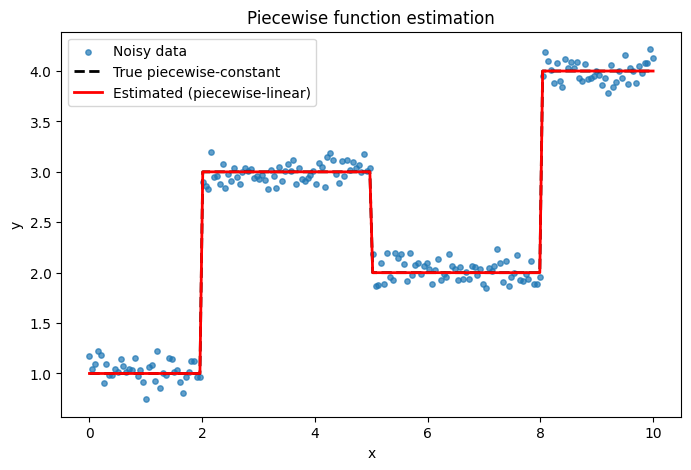
\includegraphics[width=0.7\textwidth]{figs/lam001.png}
\caption{$\lambda = 0.001$}
\end{figure}

\begin{figure}[H]
\centering
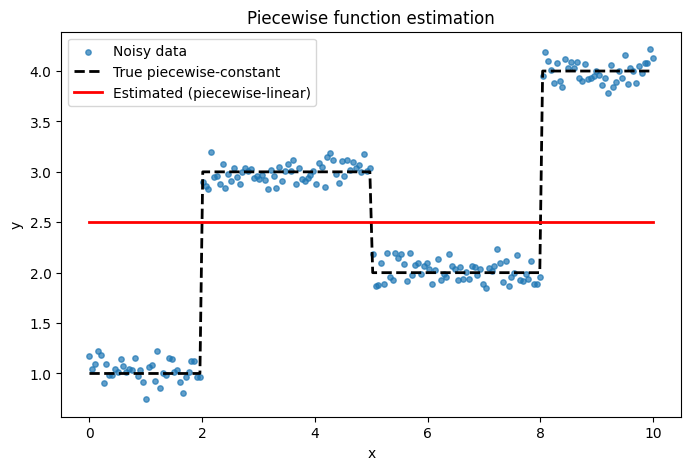
\includegraphics[width=0.7\textwidth]{figs/lam5.png}
\caption{$\lambda = 5$}
\end{figure}

Greater the value of $\lambda$, the more regularization is applied, which encourages fewer kinks and a smoother function. As $\lambda$ increases, the estimated function becomes more piecewise-constant, closely approximating the true underlying function. 
Like KNN algorithm, the choice of $\lambda$ is crucial and can be selected using techniques such as cross-validation to balance bias and variance in the model.
%----------------------------------------------------------------------------------------

\newpage
\section*{Problem 6. A review of standard problem formulations}

In this question, we review conceptually the standard forms of various problems and the assertions we can (and cannot!) make about each. The solutions are given, you just need to read them, understand them, and copy-paste them to your submission.

(a) Linear programming (LP).

(i) Write the most general form of a linear program (LP) and list its defining attributes.

Solution: A general LP can be written as

\[
p^* = \min_{\vec{x} \in \mathbb{R}^n} \vec{c}^\top \vec{x} + d
\]


\[
s.t.\quad A_{eq} \vec{x} = \vec{b}_{eq}
\]

\[
A \vec{x} \le \vec{b}.
\]

or equivalently,

\[
p^* = \min_{\vec{x} \in \mathbb{R}^n} \vec{c}^\top \vec{x} + d
\]

\[
s.t.\quad A_{eq} \vec{x} = \vec{b}_{eq}
\]

\[
\vec{x} \ge 0.
\]

The first LP formulation is known as the inequality form; the second is known as the conic form. A full treatment of the equivalence of these forms and how to convert between them can be found in Section 9.3 of Calafiore \& El Ghaoui.

(ii) Under what conditions is an LP convex?

Solution: An LP is always convex, as the objective function and all constraints are convex (affine) and all equality constraints are affine.


\vspace{30pt}
(b) Quadratic programming (QP).

(i) Write the most general form of a quadratic program (QP) and list its defining attributes.

Solution: A general QP can be written as

\[
p^* = \min_{\vec{x} \in \mathbb{R}^n} \frac{1}{2}\vec{x}^\top H \vec{x} + \vec{c}^\top \vec{x} + d
\]

subject to

\[
A_{eq} \vec{x} = \vec{b}_{eq}
\]

\[
A \vec{x} \le \vec{b}.
\]

(ii) Under what conditions is a QP convex?

Solution: A QP is convex if and only if \(H \succeq 0\) (i.e., positive semidefinite).

\vspace{30pt}
(c) Quadratically constrained quadratic programming (QCQP).

(i) Write the most general form of a quadratically-constrained quadratic program (QCQP) and list its defining attributes.

Solution: A general QCQP can be written as

\[
p^* = \min_{\vec{x}} \vec{x}^\top H_0 \vec{x} + 2\vec{c}_0^\top \vec{x} + d_0
\]

\[
s.t. \quad \vec{x}^\top H_i \vec{x} + 2\vec{c}_i^\top \vec{x} + d_i \le 0, \quad i = 1, ..., m
\]

\[
\vec{x}^\top H_j \vec{x} + 2\vec{c}_j^\top \vec{x} + d_j = 0, \quad j = 1, ..., q.
\]

(ii) Under what conditions is a QCQP convex?

Solution: A QCQP is convex if and only if all matrices \(H_0\) and \(H_i\) (for \(i = 1,...,m\)) are PSD, and \(H_j = 0\) for all equality constraints \(j = 1,...,q\) (i.e., the equality constraints are affine).


\vspace{30pt}
(d) Second-order cone programming (SOCP).

(i) Write the most general form of a second-order cone program (SOCP) and list its defining attributes.

Solution: A general SOCP can be written as

\[
p^* = \min_{\vec{x} \in \mathbb{R}^n} \vec{c}^\top \vec{x}
\]

\[
s.t. \quad \|A_i \vec{x} + \vec{b}_i\|_2 \le \vec{c}_i^\top \vec{x} + d_i, \quad i = 1,...,m.
\]

or equivalently

\[
p^* = \min_{\vec{x} \in \mathbb{R}^n} \vec{c}^\top \vec{x}
\]

\[
s.t. \quad (A_i \vec{x} + \vec{b}_i, \vec{c}_i^\top \vec{x} + d_i) \in K_{m_i}, \quad i = 1,...,m
\]

where the second-order cone is

\[
K_n = \{(\vec{x}, t) \mid \vec{x} \in \mathbb{R}^n, \ t \in \mathbb{R}, \ \|\vec{x}\|_2 \le t\}.
\]

(ii) Under what conditions is an SOCP convex?

Solution: An SOCP is always convex, as the objective function is convex (linear) and the constraint stipulates that points lie within a convex set.

\vspace{30pt}
(e) Relationships.

Recall that

\[
LP \subset QP_{convex} \subset QCQP_{convex} \subset SOCP \subset \{\text{all convex programs}\}.
\]

Which of these problems can be solved most efficiently? Why are these categorizations useful?


%----------------------------------------------------------------------------------------

\section*{Problem 7. Homework Process}

With whom did you work on this homework? List the names and SIDs of your group members.

NOTE: If you didn’t work with anyone, you can put “none” as your answer.

\subsection*{Answer}
none



%----------------------------------------------------------------------------------------
\end{document}
